
%\section{Tipps/Notes}
%  Pictures for what:
%  Aris logo ? 
%  Atmospheric model ? 
%  Different sensors ? 
%  Sensor Network
%  
%  
%  Problems found so far:
%  \begin{itemize}
%   \item How to calculate Height out of Pressure/Temp/Humidity Fabian version: $44330 * (1 - (\frac{pressure}{101325})^{ \frac{1}{5.255}})$
%   \item How to parameterize the different sensors (Measuring, Test Flight, Data Sheet ) ? 
%   \item How to fuse together Data from Sensors that have different Taus, especially those who are slower than the Loop-Time ?
%   \item How to integrate AirBreaks/Drag Force of Air/ Trust of Motor a input value?
%   \item What are the different noise factors and when do they occur ?
%   \item The up-flight is rather short: about 25 seconds, so the Fusion should have a small settling time
%   \item The Micro-Chip on which it is used is no the fastest : 168 MHz clock
%   \item The Ram on the Chip is not endless: Maximal space for the Sensor fusion is about 10kB
%   \item The Sensor Fusion should be as modular as possible so that it also can be used in the next competition
%   \item The Sensor Fusion has to be as sturdy as possible so that it will not fail if a problem occurs
%   \item The Fusion should make a state Estimation as precise as possible.
%   \item There are a lot of different variables: 3 Positions, 1 Speed, 3 Accelerations, 3 Lagen, Time, Pressure, Tempterature, Humidity, Up-/Downforce.
%   \item Especially the Input Value u which is the force onto the rocket is difficult to define (Drag, Trust = acceloration depends on wheigt which changes over time).
%   \item The different Sensor have different weaknesses: \begin{itemize}
% 							 \item Accelerometer: Offset, drift, weak to vibrations
%                                                          \item Gyro: Weak to Vibrations
%                                                          \item Barometer: Many uncertenties, unpercise
%                                                          \item GPS: Slow (max 5Hz)
%                                                         \end{itemize}
%                                                         
% 								  
%  \end{itemize}
 
 \begin{figure}[h!]
 \centering
 
\includegraphics[width=0.2\textwidth]{./Pictures/ARIS_TELL_Badge.png}
 % ARIS_TELL_Badge.png: 0x0 pixel, 300dpi, 0.00x0.00 cm, bb=
 \caption{Official logo of the competition project 2018}
 \label{fig:ArisTell}
\end{figure}

 The Academic Space Initiative Switzerland (ARIS) figure:\ref{fig:ArisTell} is a student group which tries too compete in the yearly Intercollegiate Rocket Engineering Competition (IREC).
 The goal of this competition is to build a rocket which can fly autonomous at a predefined apogee (10000 feet).
 The competitors are graded by the documentation about the project, how much of the parts they engineered/produced itself and how precises the apogee was hit. \\
 To aim for the right apogee a Control algorithm is implemented. 
 This algorithm relays on the information of different sensors to determine the rockets actual state.
 Cause there are different sensors to measure the same value a algorithm which fuses those data would come in handy.
 With this fusion algorithm it should also be possible to be more accurate as with each sensor on its own.
 The purpose of this thesis is to implement a simulation and with its help find the algorithm which is most suitable for this task.\\
 For this the problem as well as the desired solution will be defined in this chapter.
 After that the models for the different sensor that will be used as well as the pro and con of different state estimators are discussed at beginning of chapter \ref{ch:Approach}.
 In addition, different possible system models are also described in this chapter.
 Chapter \ref{ch:Implementation} will then show, how the simulation and the fusion algorithm are implemented in detail.
 To verify that the implementation is working as intended, the results of the simulation are discussed in chapter \ref{ch:Tests}.
 In the last chapter \ref{ch:Conclusion} a summary of the achieved knowledge, as well as a comparison between the desired and the implemented solution will be stated.

 
 \section{Purpose}
 The hardware as well as the most of the software parts that will be used for this competition is already defined.
 Also it is a suitable assumption that the sensors and the dynamics of the rocket will be stay more or less the same for the competitions coming.
 Therefore this thesis will mainly focus on finding a algorithm for this given surroundings, but it is also will try to find as modular solution as possible, 
 so that achieved knowledge can be used in further competition.
  
 \section{Research}
 Sensor/data fusion and state estimation is a well established engineering field.
 Especially since the 1960 when Rudolf A Kalman published his paper for the Kalman filter.
 Therefore there is already a lot of previous work which can be used in this thesis.
 For this thesis two books are used which provide the needed theory, this are by name
 \cite{DavidWSchultz2004} which contains basic theory about kalman filters. The second book
 \cite{SimonDan2006Ose:} is more focused on different approaches of state estimation and
 provides also different solution to common problems that occur while implementing a state estimation.
 In addition the Master Thesis \cite{BryanTongMinh2012} accesses more ore less the same issue as this thesis.
 Therefore it will be used mainly in the conceptional part of this paper.
 
 
 \section{Sensors}
 \begin{figure}[h!]
  \centering
  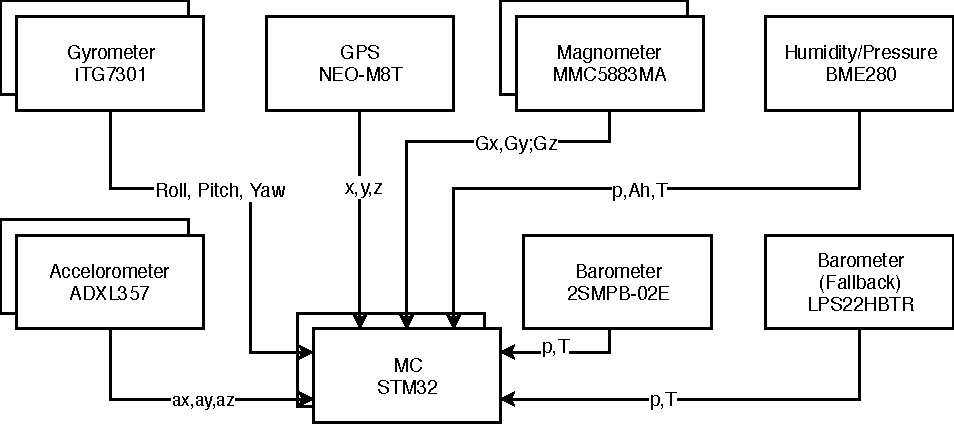
\includegraphics[width = \textwidth]{../BDADoku/Pictures/SensorNetworkAlt.pdf}
  \caption{Sensor Network}
  \label{fig:SensorNetwork}
 \end{figure}

 As mentioned above different sensors are used in this years competition.
 This used sensors and their settings will be described in this chapter.
 
 %% Maybe add pictures of the different sensors 
 \subsection{Accelerometer}
 First of all, comes the accelerometer. This is a well established and widely used sensor. It measures the force which is applied on the sensor in the three
 space dimensions. 
 This years accelerometer is adxl357 which will be sampled at 1000 Hz. It has an accuracy of bla meters per seconds squared. 
 
 \subsection{Gyrometer}
 The Gyrometer is needed to measure the posture of the Rocket. This is especially needed to determine if the rocket has a pitch angle. If so the pure
 acceleration on the z-axis can be calculated. The used gyrometer is ITG-3701.
 
 \subsection{Barometers}
 Barometers are widely used in aviation, cause with a common pressure model the height can be calculated out of the measurements that the barometer takes.
 In this years competition three barometers are used. This are by name 2SMPB-02E and LPS22HBTR. They will be used with a sampling rate 100Hz and 50Hz. %Has to be checked
 
 \subsection{Temperature}
 The temperature is maybe needed to make the height out of the barometer better because most of the atmospheric model depend on the pressure as well as the temperature.
 This temperature will be provided by the different barometers which each posses a separate temperature sensor. 
 
 \subparagraph{Magnometer}
 Also there are two Magnometer in the sensor network \ref{fig:SensorNetwork}. These measure the strengths of the surrounding magentic field.
 This can be used to determine the direction regarding the north pole.
 Due to the fact that the algorithm that will be developed in this thesis does not include the X- and Y-Axis,
 these sensor will not be used for the sensor fusion.
 
 \subsection{GPS}
 For next years competition differential GPS will be implemented with the help of two $\mu$blocks modules.
 This taken measurements are more precise as the rest of sensors but are taken much slower on a rate like 1 Hz. Therefore the algorithm should takes
 those provided measurements and interpolate between them with the data from the other sensors.
 
 
 \section{Problems}
 Out of the research and the previous competition, different problems appeared that need to be addressed in this thesis to ensure an as good solution as possible.
 
 \subsection{Different Sensors}
 First of all there are different sensors which all do measure different values and have different parameters (precision, sampling time).
 So the algorithm has to use out the strengths of the different sensors to cancel out their individual weaknesses.
 Additionally, because this algorithm is system critical, it has to be reliable enough that it still is working properly if sensors failing. 
 
 \subsection{System Load}
 The cycling time will be around 1 ms on a embedded system. This time was chosen on the behalf that it would be difficult to get the exact needed cycling time on ensure the needed controlability of the rockets apogee.
 Therefore the system load that the algorithm can cause, has to be strongly limited, so that it can be run on this given system. 
 The system this year is an 32 bit Arm Processor which runs on 168 MHz, assumed that the algorithm has at maximum the half of a software cycle, the maximum given clock cycles are around 84 000.
 With this cycles the processor can do around 10000 simple calculation (addition, subtraction, multiplication, division),
 cause with its floating point unit it needs on average around 8.5 cycles per operation (load, calculate, store). 
 This number is just a rough assumption, which means that the final system load should not exceed this value by a great manner.
 
 \subsection{Precision}
 The Precision is after the system load the most critical attribute, if the algorithm does not get into the required accuracy the whole thing is more or less for nothing.
 The Control stated that the maximal error between the estimated and ground truth height should not exceed two meter. This accuracy is needed to proper control the aim of the apogee.
 
 \subsection{Settling Time}
 The settling time defines the time span when the first reliable measurements arrive after burnout until the estimation is into the required precision.
 This time span has to be small enough to ensure that the controlling has enough time to aim for the desired apogee. In the current system the burnout occurs 
 occurs around 3-3.5 seconds after ignition, whereas the whole flight upwards only takes around 23 seconds. Therefore the settling time needs to be around just
 one second so that the control has as much time as possible for the controlling.
 
 \subsection{Reliability}
 Due to given surroundings that come if a sensor package is placed into a rocket, the assumption has to be made that it will be possible that sensors fail in execution.
 Therefore the algorithm should provide the reliability of still working in a proper manner with some sensors failed. So that the execution of the controlling software
 in terms of functionality, but locally it has not to be as accurate as it would be with all sensors working.

 \subsection{Modularity}
 Although it can be assumed that the sensors will stay more or less they same over the next competitions, it is not ensured that exactly this sensors will be used.
 Therefore the presented algorithm should provide the possibility to exchange the sensors, as long as they resemble the old sensor in a feasible way.
 This will ensure a long term use of the provided algorithm.
 
 \section{Requirements}
 
 \begin{table}[h]
 \centering
 \begin{tabular}{|l|l|l|l|}	
 \hline	
 \bf{Requirement}   & \bf{Rating} & \bf{Aim} & \bf{Importance} \\ \hline
 System Load   & \# Calculation steps per loop & < 5000 & Critical \\ \hline
 Precision     & Error between estimation and ground truth  & < 2m in Z & High  \\ \hline
 Settling time & Time from first reliable to optimal estimation  & < 1 s &  High \\ \hline
 Reliability   & Functioning Estimation with \#failed sensors & 2-3 sensors & Medium \\ \hline	
 Modularity    & Effort needed to change a sensors & < 10 h work &  Desirable \\ \hline
 \end{tabular}	
 \caption{Requirements table}
 \label{tab:Requirements}
 \end{table}
 
 As seen in the table \ref{tab:Requirements} five requirements were drown out of the problem analysis. 
 First of all, there is critical requirement the system load. This is given as critical cause it is needed that the algorithm is small enough to be run on a embedded system.
 Any solution that would not fit this requirement would be pointless in the frame of this thesis.
 Secondly there are two requirements which are tied together, the precision and settling time.
 Where the precision describes what a optimal estimation is under the context of this thesis, the settling time relies on this to be defined.
 The desired precision will be needed to ensure a possible good control.
 
 \section{Desired Solution}
 The desired solution should met the given requirements as optimal as possible. While doing this it should also not be more complicated than needed
 to make a future use as easy as possible. Cause of this the modularity is an important requirement to ensure this.
